\documentclass[11pt]{article}

\usepackage[T1]{fontenc}
\usepackage{lmodern}
\usepackage{microtype}
\usepackage[margin=1in]{geometry}
\usepackage{amsmath,amssymb,amsthm,mathtools,bm}
\usepackage{booktabs,array,tabularx}
\usepackage{graphicx}
\usepackage{xcolor}
\usepackage{enumitem}
\usepackage{natbib}
\usepackage{url}
\usepackage{hyperref}
\usepackage[nameinlink,noabbrev]{cleveref}

\graphicspath{{figures/}}
\hypersetup{
  colorlinks=true,
  linkcolor=blue!45!black,
  citecolor=blue!45!black,
  urlcolor=blue!45!black,
  pdftitle={Photo-Finish Watermarking},
  pdfauthor={Peter Cotton}
}

\setlength{\parindent}{1.2em}
\setlength{\parskip}{0.15em}
\setlist[itemize]{leftmargin=1.5em,itemsep=0.25em,topsep=0.4em}
\setlist[enumerate]{leftmargin=1.7em,itemsep=0.25em,topsep=0.4em}

\newtheorem{theorem}{Theorem}[section]
\newtheorem{proposition}[theorem]{Proposition}
\newtheorem{corollary}[theorem]{Corollary}
\newtheorem{lemma}[theorem]{Lemma}
\theoremstyle{definition}
\newtheorem{definition}[theorem]{Definition}
\theoremstyle{remark}
\newtheorem{remark}[theorem]{Remark}

\DeclareMathOperator{\diag}{diag}
\DeclareMathOperator{\softmax}{softmax}
\DeclareMathOperator{\tr}{tr}
\DeclareMathOperator{\rank}{rank}
\DeclareMathOperator{\sign}{sign}
\DeclareMathOperator{\KL}{KL}
\DeclareMathOperator{\TV}{TV}
\DeclareMathOperator{\Var}{Var}
\DeclareMathOperator{\Cov}{Cov}
\DeclareMathOperator*{\argmax}{arg\,max}
\newcommand{\R}{\mathbb{R}}
\newcommand{\E}{\mathbb{E}}
\newcommand{\Pp}{\mathbb{P}}
\newcommand{\one}{\mathbf{1}}
\newcommand{\Dp}{D_p}
\newcommand{\trans}{\mathsf{T}}

\title{\textbf{Photo-Finish Watermarking:}\\
SynthID as a Laplacian Flow and Distortion-Free Gaussian Sampling}
\author{Peter Cotton}
\date{August 2026\\[0.3em]\small Working draft --- theoretical results and synthetic verification only}

\begin{document}
\maketitle

\begin{abstract}
A non-distortionary text watermark must correlate secret randomness with the selected token while preserving the model's next-token distribution after averaging over that randomness. We identify an exact graph structure underneath the two-sample Tournament layer used by SynthID-Text and use it to construct a Gaussian analogue. For a base distribution $p$ and token scores $g$, one Tournament layer is an oriented flow on the complete graph with edge conductances $p_i p_j$. When $g\in\{0,1\}^N$, the flow linearizes exactly:
\[
q=p+J_{\rm sm}(p)g,
\qquad
J_{\rm sm}(p)=\diag(p)-pp^\trans,
\]
so non-distortion is the null-space identity $J_{\rm sm}\one=0$. The keyed score gain, conditional total variation, and Pearson $\chi^2$ displacement all equal the same Dirichlet energy $a(1-a)$, where $a=p^\trans g$. Iterated layers form a probability-vector martingale; their collision probability rises and the expected capacity of the next random cut falls, giving a graph explanation of SynthID's diminishing layer strength.

The Gaussian construction begins with a low-rank-plus-diagonal perturbed maximum. Given target shares $p$ and covariance $\Sigma=VV^\trans+\diag(D)$, a companion share-inversion algorithm produces the unique mean-zero utility vector $\mu_\Sigma(p)$. We expose a fraction $\rho$ of the factor shock to the secret key and leave the remainder as fresh sampling noise:
\[
Y=\argmax_i\left\{\mu_i+\sqrt{\rho}\,v_i^\trans R
       +\sqrt{1-\rho}\,v_i^\trans Z+\sqrt{D_i}\,\epsilon_i\right\}.
\]
For every $\rho\in[0,1]$, the marginal law of $Y$ is exactly $p$. Larger $\rho$ Blackwell-dominates smaller $\rho$: both mutual information with the key and same-key posterior collision are nondecreasing. The likelihood-ratio detector has expected evidence $I(R;Y)$. A detector not requiring the language-model probabilities uses the score $R^\trans v_Y$; Gaussian integration by parts shows that its watermark drift is the Dirichlet energy of the exposed loading field on the conditional photo-finish graph. Under ideal independent context seeds, its standardized null distribution is exactly normal, not merely asymptotically normal.

Locally, detection information is governed by $J\diag(p)^{-1}J$, while Gaussian mirror movement is governed by the photo-finish Laplacian $J$ or, in share coordinates, its effective-resistance inverse $J^+$. Softmax is the exceptional case in which these geometries coincide. Synthetic experiments verify the identities to numerical precision. No language-model quality, robustness, or production-latency claim is made: current share inversion is too slow for full-vocabulary autoregressive deployment, and the paper ends with the experiments needed to decide whether the construction is useful in practice.
\end{abstract}

\noindent\textbf{Keywords:} language-model watermarking; SynthID-Text; multinomial probit; perturbed maximum; graph Laplacian; effective resistance; Gaussian coupling; distortion-free sampling

\section{Introduction}

A generative text watermark is a coupling problem. At one decoding step, a language model supplies a categorical distribution $p$ over a vocabulary. A secret-key mechanism supplies side information $R$. The watermarked sampler must produce a token $Y$ that is statistically dependent on $R$, because that dependence is the evidence available to a detector, while preserving the desired output law after the key randomness is averaged out:
\begin{equation}
  \Pp(Y=i)=\E_R\big[\Pp(Y=i\mid R)\big]=p_i.
  \label{eq:nondist-intro}
\end{equation}
This is the single-token form of non-distortion. It does not say that the conditional distribution given a particular key is unchanged. On the contrary, a useful watermark makes those conditional distributions different and arranges their average to be exactly $p$.

This viewpoint is explicit in distortion-free and cryptographically undetectable watermarking \citep{kuditipudi2024robust,christ2024undetectable,hu2024unbiased,tsur2025couplings}. It is also the operative principle of SynthID-Text \citep{dathathri2024synthid}. SynthID's Tournament sampler repeatedly draws pairs of candidates, lets keyed token scores determine each pair's winner, and samples from the final tournament distribution. Its non-distortion theorem is already established, as is a detailed collision-entropy analysis in the supplementary material. The first observation of this paper is therefore not a new watermarking algorithm. It is an exact identification of the algorithm's geometry.

For two candidates, the probability that the unordered pair $\{i,j\}$ is drawn is $2p_i p_j$. Relative to drawing one token from $p$, the tournament transfers $p_i p_j$ units of probability from the lower-scoring token to the higher-scoring token. Thus one layer is an oriented flow on the complete graph whose conductances are $p_i p_j$. These are exactly the conductances of the softmax Jacobian
\[
J_{\rm sm}(p)=\diag(p)-pp^\trans.
\]
For binary keyed scores, edge orientation equals the score difference, so the entire nonlinear tournament reduces to the exact linear identity
\begin{equation}
q=p+J_{\rm sm}(p)g.
\label{eq:headline-synthid}
\end{equation}
The matrix in \eqref{eq:headline-synthid} is simultaneously the Hessian of log-sum-exp, the Fisher information of a categorical softmax model, and the weighted graph Laplacian of what the companion work calls the \emph{photo-finish graph}. The SynthID layer is therefore a softmax photo-finish flow driven by a secret random voltage.

The second observation runs in the opposite direction. The Gumbel-max trick samples exactly from $p$ by adding keyed Gumbel shocks to $\log p$ and taking an argmax. Gaussian perturbations should offer a correlated and low-rank analogue, but a Gaussian race does not map $\log p$ to $p$. One must first solve the multinomial probit inverse problem: for a fixed Gaussian covariance $\Sigma$, find utilities $\mu$ whose winner probabilities equal $p$. That inverse is the computational object supplied by \citet{cotton2026calibration}. For low-rank-plus-diagonal covariance, it is globally well posed and can be evaluated without simulation.

Once this inverse exists, an exact watermark follows from the tower property. Split a Gaussian shock into a keyed component and an independent private component. Calibrate $\mu$ to the law of their sum. The detector knows the keyed component; the generator additionally samples the private component. The conditional token distribution carries watermark information, but its key average is exactly the calibrated distribution. The stability of the Gaussian law under covariance splitting gives a continuous parameter $\rho$ controlling how much of the perturbation is exposed to the key without changing the marginal token law at all.

\subsection{Contributions and novelty boundary}

The paper makes six claims, separated deliberately from what is already known.

\begin{enumerate}
\item \textbf{Graph form of Tournament sampling.} A two-sample Tournament layer is an oriented complete-graph flow. In the binary case, SynthID's supplementary Equation E20 becomes exactly \eqref{eq:headline-synthid}. This is a reinterpretation and a source of short corollaries, not a claim to have invented Tournament sampling or its non-distortion proof.

\item \textbf{Exact conditional identities.} For a binary layer, the keyed mean-score gain, $\TV(q,p)$, and $\chi^2(q\|p)$ all equal the random-cut Dirichlet energy $a(1-a)$. The conditional distribution is also an exact two-level softmax tilt. Existing SynthID results on collision probability and diminishing layer strength become graph-capacity statements.

\item \textbf{Calibrated Gaussian factor watermark.} We propose to expose part of a factor-Gaussian perturbation to the key while keeping the total covariance fixed. Probit share inversion supplies the required mirror map $p\mapsto\mu_\Sigma(p)$. To our knowledge, this calibrated correlated-Gaussian construction has not previously been proposed for text watermarking.

\item \textbf{Detection and information geometry.} The optimal model-aware evidence is a conditional likelihood ratio with mean $I(R;Y)$. A model-free linear score has drift equal to photo-finish Dirichlet energy by Stein's identity and has an exact Gaussian null under ideal independent context seeds. Locally, the likelihood geometry $J\diag(p)^{-1}J$ separates from the mirror/effective-resistance geometry $J^+$; softmax is the case in which they collapse.

\item \textbf{Detection-optimal exposure is an eigenproblem.} Among
unit directions in factor space, the keyed drift of the directional
score is the Rayleigh quotient of $M=\E_R[V^\trans J_{\rho,R}V]$, so
the best watermark direction is the principal eigenvector of a
$k\times k$ matrix assembled from photo-finish conductances
(\cref{thm:eigen}).

\item \textbf{Reproducible synthetic verification and a falsifiable program.} Seeded experiments verify every new algebraic and Gaussian identity and illustrate the key-exposure frontier. They do not test an LLM. The practical case remains to be established against modern distortion-free systems, including SynthID-Text and Gumbel-based methods such as TextSeal \citep{sander2026textseal}.
\end{enumerate}

Recent work has already sharpened the analysis of SynthID-Text. In particular, \citet{omidi2026synthid} study detection, layer inflation, and the optimal Bernoulli parameter for their criterion. Accordingly, this paper does not claim novelty for choosing Bernoulli$(1/2)$, for the fact that later Tournament layers weaken, or for the broader coupling formulation of distortion-free watermarking. Its proposed new object is the Gaussian factor coupling and the photo-finish geometry connecting it to SynthID.

\section{Perturbed maxima and photo-finish graphs}
\label{sec:background}

Let $\Delta_N^\circ=\{p\in\R^N:p_i>0,\ \one^\trans p=1\}$, and let $e_i$ be the $i$th coordinate vector. A random-utility choice model takes
\begin{equation}
Y=\argmax_{1\le i\le N}\{\mu_i+\xi_i\},
\label{eq:random-utility}
\end{equation}
with a continuous shock vector $\xi$. Define the social-surplus potential and choice map
\begin{equation}
G(\mu)=\E\max_i(\mu_i+\xi_i),
\qquad
p(\mu)=\nabla G(\mu).
\label{eq:wdz}
\end{equation}
The gradient identity is the Williams--Daly--Zachary/McFadden identity \citep{mcfadden1981probabilistic}; in machine learning it organizes differentiable perturbed optimizers \citep{berthet2020perturbed}. Translation leaves choices unchanged, so $p(\mu+c\one)=p(\mu)$ and the Jacobian $J=\nabla^2G$ satisfies $J\one=0$.

For independent Gumbel shocks, $G$ is log-sum-exp and $p=\softmax(\mu)$. Writing $\Dp=\diag(p)$,
\begin{equation}
J_{\rm sm}(p)=\Dp-pp^\trans
=\sum_{i<j}p_i p_j(e_i-e_j)(e_i-e_j)^\trans.
\label{eq:softmax-laplacian}
\end{equation}
Thus the softmax Jacobian is the Laplacian of a complete graph with conductances $w_{ij}=p_i p_j$.

The same structure holds more generally. In the factor-Gaussian model
\begin{equation}
U_i=\mu_i+v_i^\trans f+\sqrt{D_i}\,\epsilon_i,
\qquad
f\sim N(0,I_k),\quad \epsilon_i\stackrel{\rm iid}{\sim}N(0,1),\quad D_i>0,
\label{eq:factor-probit}
\end{equation}
conditional independence gives the all-alternatives winner formula
\begin{equation}
p_i(\mu)=\E_f\int g_i(x\mid f)\prod_{j\ne i}F_j(x\mid f)\,dx.
\label{eq:shared-field}
\end{equation}
Here $F_i$ and $g_i$ are the conditional CDF and density. Differentiation yields
\begin{equation}
J(\mu)=\sum_{i<j}w_{ij}(\mu)(e_i-e_j)(e_i-e_j)^\trans,
\quad
w_{ij}=\E_f\int g_i g_j\prod_{\ell\ne i,j}F_\ell\,dx>0.
\label{eq:general-photo-finish}
\end{equation}
The weight $w_{ij}$ is the density of an $i$--$j$ tie at the winning frontier with every other alternative behind: a photo finish. The graph is complete and connected, so $J$ is positive definite on $\one^\perp$. The map $\mu\mapsto p$ is consequently a diffeomorphism from the mean-zero quotient to $\Delta_N^\circ$ for fixed $(V,D)$ \citep{cotton2026calibration}.

Let $\Psi=G^*$ be the convex conjugate restricted to the simplex. In the mean-zero gauge,
\begin{equation}
p=\nabla G(\mu),\qquad \mu=\nabla\Psi(p),\qquad \nabla^2\Psi(p)=J^+,
\label{eq:mirror-map}
\end{equation}
where $J^+$ is the Moore--Penrose pseudoinverse on $\one^\perp$. For a transfer direction $d_{ij}=e_i-e_j$,
\begin{equation}
d_{ij}^\trans J^+d_{ij}
\label{eq:resistance}
\end{equation}
is the effective electrical resistance between $i$ and $j$ in the photo-finish network \citep{cotton2026gaussian}. For softmax this resistance is $1/p_i+1/p_j$, the curvature of negative Shannon entropy along the same transfer.

\section{SynthID-Text as an exact graph flow}
\label{sec:synthid}

We analyze one two-candidate Tournament layer. Let $A,B\stackrel{\rm iid}{\sim}p$. A keyed score vector $g=(g_1,\ldots,g_N)$ assigns a real score to every token. The layer outputs the candidate with the larger score; ties between distinct candidates are broken uniformly. Let $q(g)$ denote the resulting token distribution conditional on $g$.

Fix an arbitrary orientation of the complete graph, with edge vector $b_{ij}=e_i-e_j$ for $i<j$. Define $\sign(0)=0$.

\begin{theorem}[Tournament flow on the softmax graph]
\label{thm:tournament-flow}
For every $p\in\Delta_N$ and score vector $g\in\R^N$,
\begin{equation}
q(g)-p
=\sum_{i<j}p_i p_j\,\sign(g_i-g_j)(e_i-e_j).
\label{eq:oriented-flow}
\end{equation}
Consequently,
\begin{equation}
g^\trans(q(g)-p)
=\sum_{i<j}p_i p_j\,|g_i-g_j|\ge 0.
\label{eq:score-total-variation}
\end{equation}
If the coordinates of $g$ are iid from any common distribution, then $\E_g[q(g)]=p$.
\end{theorem}

The proof is pair accounting. When $i\ne j$ are the two candidates, the tournament outcome differs from a fair selection between the two by transferring $p_i p_j$ of unconditional probability from the lower-scoring endpoint to the higher-scoring endpoint. Symmetry of iid keyed scores gives $\E\sign(g_i-g_j)=0$ on every edge. This supplies a one-line graph proof of the single-layer two-sample non-distortion theorem of \citet{dathathri2024synthid}.

The flow in \eqref{eq:oriented-flow} uses the same conductances $p_i p_j$ as the softmax photo-finish graph, but it saturates each edge according to the rank ordering of the scores. The binary case is special because saturation becomes linear.

\begin{corollary}[Binary SynthID layer]
\label{cor:binary-layer}
Suppose $g\in\{0,1\}^N$ and set
\begin{equation}
a=p^\trans g=\sum_i p_i g_i.
\end{equation}
Then
\begin{equation}
q_i=p_i(1+g_i-a),
\qquad
q=p+J_{\rm sm}(p)g.
\label{eq:binary-laplacian}
\end{equation}
This is SynthID's vectorized two-sample, one-layer formula written as a Laplacian flow.
\end{corollary}

Indeed, on a binary edge, $\sign(g_i-g_j)=g_i-g_j$. Substitution into \eqref{eq:oriented-flow} gives \eqref{eq:binary-laplacian} by \eqref{eq:softmax-laplacian}. The non-distortion identity for iid Bernoulli$(\theta)$ keys is now
\begin{equation}
\E_g[q]
=p+J_{\rm sm}\E[g]
=p+\theta J_{\rm sm}\one=p.
\label{eq:nullspace-nondist}
\end{equation}
In words: the average secret voltage is constant, and a graph Laplacian cannot see a constant voltage.

\subsection{One scalar is simultaneously signal and conditional displacement}

The binary formula has several exact consequences not apparent from the tournament description.

\begin{proposition}[Energy, total variation, and Pearson displacement]
\label{prop:binary-metrics}
For a binary layer with cut mass $a=p^\trans g$,
\begin{equation}
\begin{split}
\E_{Y\sim q}[g_Y]-\E_{Y\sim p}[g_Y]
&=g^\trans J_{\rm sm}g\\
&=a(1-a)\\
&=\TV(q,p)\\
&=\chi^2(q\|p),
\end{split}
\label{eq:four-equalities}
\end{equation}
where $\chi^2(q\|p)=\sum_i(q_i-p_i)^2/p_i$. When $0<a<1$,
\begin{equation}
q=\softmax(\log p+\beta(a)g),
\qquad
\beta(a)=\log\frac{2-a}{1-a}.
\label{eq:adaptive-softmax-tilt}
\end{equation}
Moreover,
\begin{equation}
\KL(q\|p)
=a(2-a)\log(2-a)+(1-a)^2\log(1-a).
\label{eq:binary-kl}
\end{equation}
\end{proposition}

Thus a key-conditioned SynthID layer is not merely analogous to a softmax perturbation. It is exactly an adaptive two-level logit tilt. The adaptation of $\beta$ to the random cut mass is what permits a nonzero conditional tilt while preserving $p$ after averaging over keys. Equation \eqref{eq:four-equalities} should not be misread as a quality statement: non-distortion concerns the key average, whereas $\TV(q,p)$ is a conditional displacement for a particular key. It does show that the elementary mean-score signal and two standard measures of conditional movement are the same graph quantity.

For general iid score values $G_i$, \cref{thm:tournament-flow} gives
\begin{equation}
\E_g\left[\E_{Y\sim q(g)}g_Y-\E_{Y\sim p}g_Y\right]
=\frac{1-C_2(p)}{2}\,\E|G-G'|,
\label{eq:general-score-gain}
\end{equation}
where $C_2(p)=\sum_i p_i^2$ is collision probability and $G,G'$ are iid score draws. Bernoulli$(\theta)$ gives
\begin{equation}
\E_g[g^\trans J_{\rm sm}g]
=\theta(1-\theta)\big(1-C_2(p)\big).
\label{eq:bernoulli-expected-energy}
\end{equation}
The factor $1-C_2(p)$ is the total conductance of the softmax graph, up to a factor of two. It is also the probability that two independent candidates are distinct. The choice $\theta=1/2$ maximizes this particular mean-score/Dirichlet criterion, consistently with the more detailed detection analysis of \citet{omidi2026synthid}.

\subsection{Multiple layers: a simplex martingale consuming cut capacity}

Let $p^{(0)}=p$, and apply independent binary layers recursively:
\begin{equation}
p^{(\ell)}=p^{(\ell-1)}
+J_{\rm sm}\!\left(p^{(\ell-1)}\right)g_\ell.
\label{eq:layer-recurrence}
\end{equation}
This is exactly the vectorized implementation in the SynthID supplement. Conditional on the preceding layers,
\begin{equation}
\E[p^{(\ell)}\mid p^{(\ell-1)}]=p^{(\ell-1)},
\label{eq:simplex-martingale}
\end{equation}
so the evolving conditional distribution is a martingale in the simplex. Convex functions of a martingale are submartingales; in particular, collision probability increases on average. A direct calculation gives the exact increment for iid Bernoulli$(\theta)$ scores:
\begin{equation}
\E\!\left[C_2(p^{(\ell)})\mid p^{(\ell-1)}=p\right]
=C_2(p)+\theta(1-\theta)
\left(C_2(p)+C_2(p)^2-2C_3(p)\right),
\label{eq:collision-increment}
\end{equation}
where $C_3(p)=\sum_i p_i^3$. The bracket is nonnegative because
\begin{equation}
C_2+C_2^2-2C_3
=\sum_i p_i^2(1-p_i)^2+2\sum_{i<j}p_i^2p_j^2,
\label{eq:collision-positive}
\end{equation}
with equality only at a point mass. For $\theta=1/2$, \eqref{eq:collision-increment} is the Bernoulli specialization of the collision formula in the SynthID supplementary analysis.

The expected score contribution of the next layer, conditional on its input distribution, is
\begin{equation}
s(p)=\theta(1-\theta)(1-C_2(p)).
\label{eq:next-layer-signal}
\end{equation}
Therefore \eqref{eq:collision-increment} implies that $\E s(p^{(\ell)})$ is nonincreasing. The graph interpretation is literal: each layer pushes the conditional distribution toward the simplex boundary, reducing the total conductance available to the next random cut. This is the photo-finish version of the known fact that Tournament layers consume collision entropy and have diminishing strength.

\begin{figure}[t]
\centering
\begin{minipage}[t]{0.49\textwidth}
\centering
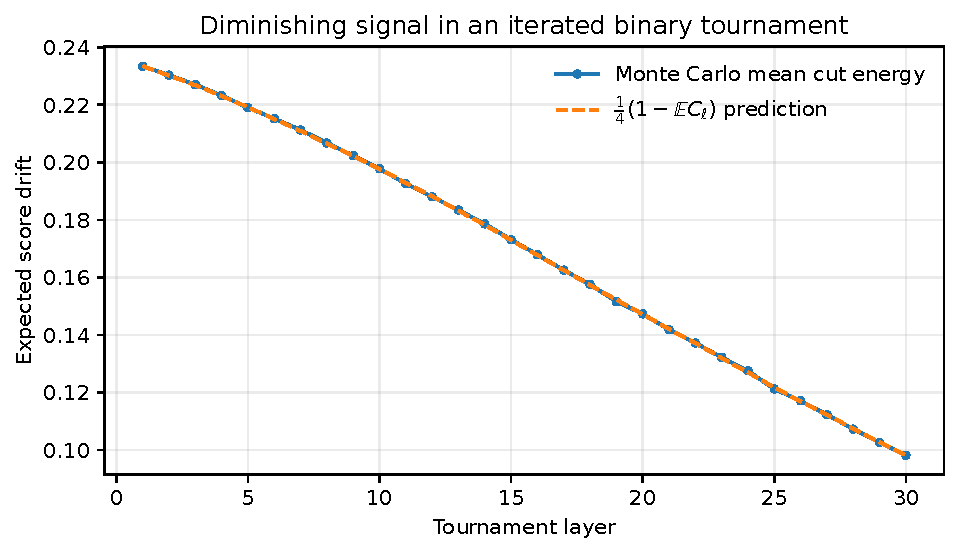
\includegraphics[width=\linewidth]{synthid_layer_signal.pdf}
\end{minipage}\hfill
\begin{minipage}[t]{0.49\textwidth}
\centering
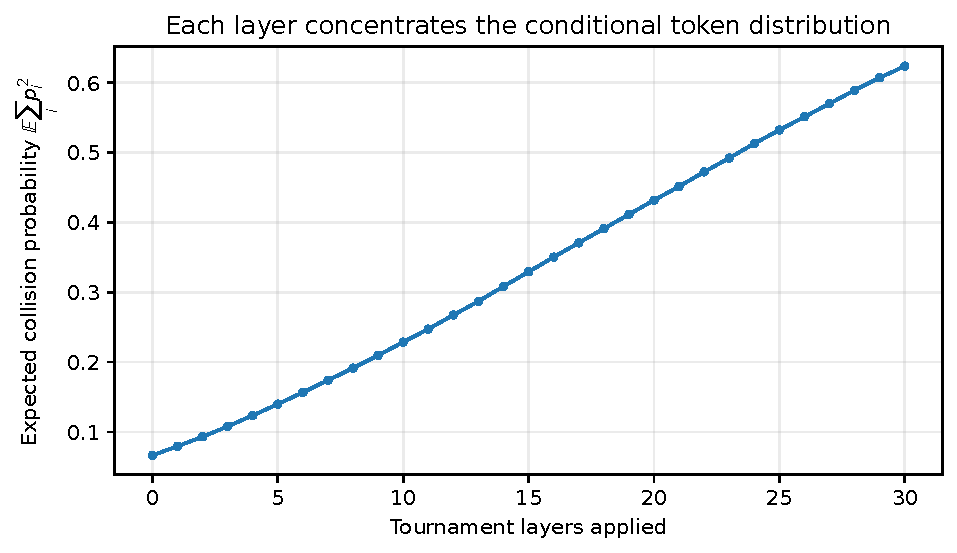
\includegraphics[width=\linewidth]{synthid_layer_collision.pdf}
\end{minipage}
\caption{\textbf{Iterated binary Tournament layers in a synthetic $N=120$ example.}
Left: the expected random-cut energy decreases over 30 layers; the dashed curve is the exact conditional prediction $\tfrac14(1-\E C_2)$. Right: the expected collision probability of the conditional token distribution rises. Each point averages 20,000 independent tournament paths. These plots illustrate known SynthID entropy behavior in the photo-finish coordinates of \eqref{eq:layer-recurrence}.}
\label{fig:synthid-layers}
\end{figure}

\section{Laplacian couplings beyond the tournament}
\label{sec:laplacian-couplings}

The binary SynthID identity suggests an abstract construction. Let
\begin{equation}
L=\sum_{i<j}w_{ij}(e_i-e_j)(e_i-e_j)^\trans
\label{eq:abstract-laplacian}
\end{equation}
be any graph Laplacian, possibly depending on the base distribution and context. Let $h$ be a keyed random voltage. Whenever
\begin{equation}
q_h=p+Lh\in\Delta_N,
\label{eq:linear-coupling}
\end{equation}
we obtain an exact keyed categorical coupling.

\begin{proposition}[Laplacian coupling lemma]
\label{prop:laplacian-coupling}
If $\E[h]\in\operatorname{span}\{\one\}$ and \eqref{eq:linear-coupling} is feasible almost surely, then $\E[q_h]=p$. If the detector scores token $i$ by $h_i$, its conditional gain is
\begin{equation}
h^\trans(q_h-p)=h^\trans Lh
=\sum_{i<j}w_{ij}(h_i-h_j)^2\ge 0.
\label{eq:laplacian-score}
\end{equation}
\end{proposition}

The construction is algebraic, not an assertion that every finite perturbation of a random-utility model is linear. For a general photo-finish graph, $J$ is the local derivative of the choice map; $p(\mu+h)$ is not normally equal to $p(\mu)+Jh$. SynthID's binary two-sample layer is exceptional because it realizes the finite linear update exactly with $L=J_{\rm sm}(p)$.

The lemma nevertheless isolates the watermarking mechanism: a secret voltage creates probability current; translation invariance places constants in the null space; the detector measures the energy dissipated by the induced current. The Gaussian construction below retains this picture, but the conditional map is nonlinear and exact non-distortion comes from a covariance decomposition rather than from a finite Laplacian step.

\section{A calibrated Gaussian factor watermark}
\label{sec:gaussian-watermark}

\subsection{Keying part of a perturbation}

The basic construction is distribution-free.

\begin{theorem}[Partial-perturbation watermark]
\label{thm:partial-perturbation}
Let $K,Z\in\R^N$ be independent random vectors such that $K+Z$ has a continuous distribution. Suppose $\mu$ is calibrated so that
\begin{equation}
\Pp\!\left(\argmax_i\{\mu_i+K_i+Z_i\}=j\right)=p_j.
\label{eq:calibrated-total}
\end{equation}
Treat $K$ as keyed side information available to the detector and $Z$ as fresh private randomness. Define
\begin{equation}
q_k(j)=\Pp\!\left(\argmax_i\{\mu_i+k_i+Z_i\}=j\right).
\label{eq:conditional-qk}
\end{equation}
Then
\begin{equation}
\E_K[q_K]=p.
\label{eq:tower-nondist}
\end{equation}
\end{theorem}

The proof is the tower property. The content lies in finding a perturbation family with a useful split, a tractable conditional law, and an attainable inverse map from $p$ to $\mu$. Gaussian perturbations supply all three in the low-rank-plus-diagonal regime.

\subsection{Covariance exposure}

Fix $V\in\R^{N\times k}$ and $D\in\R_{++}^N$, with total covariance
\begin{equation}
\Sigma=VV^\trans+\diag(D).
\label{eq:total-covariance}
\end{equation}
Let $\mu=\mu_\Sigma(p)$ be the unique mean-zero utility vector whose Gaussian winner shares are $p$. Existence, uniqueness, and a sampling-free algorithm for this mirror map are established in \citet{cotton2026calibration}.

For a key-exposure parameter $\rho\in[0,1]$, draw
\begin{equation}
R,Z\stackrel{\rm iid}{\sim}N(0,I_k),
\qquad
\epsilon\sim N(0,I_N),
\label{eq:gaussian-draws}
\end{equation}
independently, and output
\begin{equation}
Y_\rho
=\argmax_i\left\{
\mu_i+\sqrt{\rho}\,v_i^\trans R
+\sqrt{1-\rho}\,v_i^\trans Z
+\sqrt{D_i}\,\epsilon_i
\right\}.
\label{eq:gaussian-watermark}
\end{equation}
The detector regenerates $R$ from the secret key and context. The variables $Z$ and $\epsilon$ are fresh generation randomness. Conditional on $R=r$, the winner law is the residual Gaussian race
\begin{equation}
q_{\rho,r}
=p_{(1-\rho)VV^\trans+\diag(D)}
\left(\mu+\sqrt{\rho}\,Vr\right).
\label{eq:conditional-gaussian-q}
\end{equation}

\begin{corollary}[Exact Gaussian non-distortion]
\label{cor:gaussian-nondist}
For every $\rho\in[0,1]$,
\begin{equation}
\E_R[q_{\rho,R}]=p.
\label{eq:gaussian-nondist}
\end{equation}
\end{corollary}

The reason is stronger than an approximation: the combined factor
\begin{equation}
F_\rho=\sqrt{\rho}\,R+\sqrt{1-\rho}\,Z
\end{equation}
has the same $N(0,I_k)$ distribution for every $\rho$. Thus the unconditional utility vector in \eqref{eq:gaussian-watermark} always has covariance \eqref{eq:total-covariance}, the covariance used to calibrate $\mu$.

At $\rho=0$, the key is irrelevant and generation is the ordinary calibrated factor-probit sampler. At $\rho=1$, the entire low-rank factor is exposed to the key, while the diagonal residual $\sqrt{D_i}\epsilon_i$ preserves conditional randomness and smooth winner probabilities. More general Gaussian splits $\Sigma=\Sigma_K+\Sigma_0$ are immediate; the factor split is attractive because the keyed variable has dimension $k\ll N$.

\subsection{A precise evidence--diversity ordering}

The parameter $\rho$ does not change the marginal token distribution, but it changes how informative the key is about the total factor. This gives a monotone frontier.

Let
\begin{equation}
I_\rho=I(R;Y_\rho)
=\E_R\KL(q_{\rho,R}\|p),
\label{eq:rho-mi}
\end{equation}
and define posterior collision
\begin{equation}
C_\rho=\E_R\sum_i q_{\rho,R}(i)^2.
\label{eq:posterior-collision}
\end{equation}
The latter is the probability that two independent draws using the same key-side variable $R$ agree, averaged over $R$. It decomposes as
\begin{equation}
C_\rho-\sum_i p_i^2
=\E_R\|q_{\rho,R}-p\|_2^2.
\label{eq:collision-excess}
\end{equation}
Thus excess posterior collision is both a dependence measure and a one-token proxy for loss of same-key response diversity.

\begin{theorem}[Blackwell monotonicity of key exposure]
\label{thm:blackwell}
If $0\le\rho_1\le\rho_2\le1$, then the observation of the factor supplied at exposure $\rho_1$ is a Gaussian garbling of the observation supplied at exposure $\rho_2$. Consequently,
\begin{equation}
I_{\rho_1}\le I_{\rho_2},
\qquad
C_{\rho_1}\le C_{\rho_2}.
\label{eq:blackwell-monotonicity}
\end{equation}
\end{theorem}

Equivalently, if $F\sim N(0,I_k)$ denotes the total factor, the detector's side information can be represented as
\begin{equation}
R_\rho=\sqrt{\rho}\,F+\sqrt{1-\rho}\,N.
\label{eq:observation-channel}
\end{equation}
For $\rho_1\le\rho_2$, one obtains $R_{\rho_1}$ from $R_{\rho_2}$ by adding independent Gaussian noise. The mutual-information claim is data processing. The collision claim follows because posterior probabilities under the noisier observation are conditional averages of the posterior probabilities under the more informative observation, and squared Euclidean norm is convex.

The theorem formalizes a trade-off that distortion-free watermarking cannot remove: more evidence about the selected token is obtained by making the token more predictable from the key. The marginal distribution remains exactly fixed, but conditional diversity falls. Recent Gumbel-based work explicitly addresses this tension with additional keying structure \citep{sander2026textseal}; the Gaussian split exposes it as a continuous Blackwell order.

\begin{figure}[t]
\centering
\begin{minipage}[t]{0.49\textwidth}
\centering
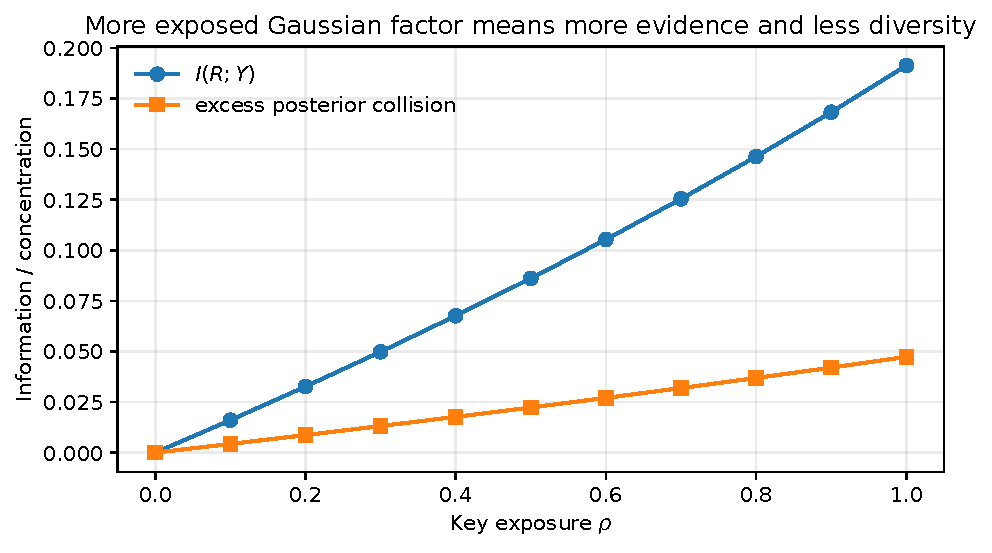
\includegraphics[width=\linewidth]{gaussian_key_exposure.pdf}
\end{minipage}\hfill
\begin{minipage}[t]{0.49\textwidth}
\centering
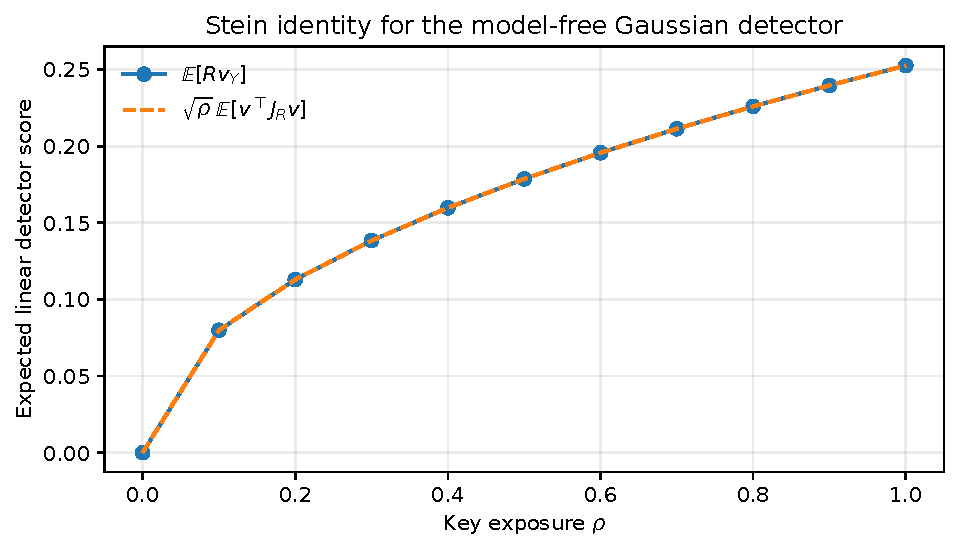
\includegraphics[width=\linewidth]{gaussian_stein_score.pdf}
\end{minipage}
\caption{\textbf{Gaussian key exposure in a synthetic ten-token race.}
Left: mutual information and excess posterior collision increase with $\rho$, while the marginal token distribution is unchanged to numerical precision. Right: the mean linear detector score agrees with the photo-finish Dirichlet energy predicted by Stein's identity. The example is a one-factor Gaussian race calibrated to a fixed target distribution; it is not an LLM experiment.}
\label{fig:gaussian-exposure}
\end{figure}

\subsection{Generation algorithm}

The mathematical sampler can be summarized as follows. The phrase ``Gaussian PRF'' means a cryptographic pseudorandom function whose output bits are deterministically mapped to approximately standard-normal coordinates.

\medskip
\noindent\fbox{\begin{minipage}{0.94\textwidth}
\textbf{Gaussian photo-finish generation at one context}
\begin{enumerate}[label=\arabic*.,leftmargin=1.5em]
\item Compute the active-support distribution $p$, and choose public $V,D$ and exposure $\rho$.
\item Obtain $\mu=\mu_{VV^\trans+\diag(D)}(p)$ by Gaussian share inversion.
\item Generate $R=\operatorname{GaussianPRF}(\text{secret key},\text{context})\in\R^k$.
\item Draw fresh $Z\sim N(0,I_k)$ and $\epsilon\sim N(0,I_N)$.
\item Return the token maximizing \eqref{eq:gaussian-watermark}.
\end{enumerate}
For model-free detection, regenerate $R$ and add the score $R^\trans v_Y$. For likelihood-ratio detection, additionally evaluate $q_{\rho,R}(Y)$ and $p_Y$.
\end{minipage}}
\medskip

The active-support qualification matters. The inverse map is finite for strictly positive target shares. A top-$k$ or top-$p$ decoder can apply the construction to its renormalized support, in which case non-distortion is exact relative to that truncated base sampler, not relative to the untruncated full softmax.

\section{Detection}
\label{sec:detection}

\subsection{The model-aware likelihood ratio}

Under the unwatermarked null, the secret side information is independent of the token and $Y\sim p$. Under the Gaussian watermark, the joint law is $dP_R(r)q_{\rho,r}(y)$. The one-token log-likelihood ratio is therefore
\begin{equation}
\ell_\rho(r,y)=\log\frac{q_{\rho,r}(y)}{p_y}.
\label{eq:llr}
\end{equation}
Its expected value under the watermark is exactly
\begin{equation}
\E_1[\ell_\rho(R,Y)]
=\E_R\KL(q_{\rho,R}\|p)
=I(R;Y).
\label{eq:llr-mi}
\end{equation}
No additive score can have greater asymptotic testing efficiency when the conditional distributions are known. Computing \eqref{eq:llr}, however, requires the base probabilities and the conditional Gaussian winner probabilities, so it is a model-aware detector.

For a sequence with independently keyed, nonrepeated contexts, the conditional log-likelihood ratios add. In a practical autoregressive system, both $p_t$ and $q_{t,r_t}$ vary with context; the exact statistic is
\begin{equation}
L_T=\sum_{t\in\mathcal T}
\log\frac{q_{t,r_t}(x_t)}{p_t(x_t)},
\label{eq:sequence-llr}
\end{equation}
where $\mathcal T$ excludes masked repeated contexts. The computational burden of evaluating $q_{t,r_t}$ is one reason to seek a detector that uses only the key, the observed token, and fixed public loading metadata.

\subsection{A model-free Gaussian score}

Let $J_{\rho,r}$ be the Jacobian of the residual winner map in \eqref{eq:conditional-gaussian-q} with respect to its mean vector. It is a photo-finish Laplacian of the form \eqref{eq:general-photo-finish}. Consider the scalar score
\begin{equation}
S(r,y)=r^\trans v_y,
\label{eq:linear-score}
\end{equation}
where $v_y$ is the row of $V$ associated with the observed token.

\begin{theorem}[Stein photo-finish identity]
\label{thm:stein}
Under the Gaussian factor watermark \eqref{eq:gaussian-watermark},
\begin{equation}
\begin{split}
\E_1[S(R,Y)]
&=\sqrt{\rho}\,\E_R\tr\!\left(V^\trans J_{\rho,R}V\right)\\
&=\sqrt{\rho}\,\E_R
\sum_{i<j}w_{ij}(R)\|v_i-v_j\|_2^2.
\end{split}
\label{eq:stein-energy}
\end{equation}
Under the unwatermarked null, $\E_0[S(R,Y)]=0$. If $D_i>0$ and the rows of $V$ are not all equal, the watermark drift is strictly positive for every $\rho>0$.
\end{theorem}

The proof uses multivariate Gaussian integration by parts \citep{stein1981mean}. Conditional on $R=r$,
\begin{equation}
\E[S\mid R=r]=r^\trans V^\trans q_{\rho,r}.
\end{equation}
Differentiating the conditional probabilities with respect to $r$ gives
\begin{equation}
\nabla_r q_{\rho,r}=\sqrt{\rho}\,J_{\rho,r}V.
\end{equation}
Stein's identity converts the factor $r$ in the expectation into this derivative, yielding \eqref{eq:stein-energy}. The common-loading gauge $V\mapsto V+\one a^\trans$ contributes no energy, so $V$ should be column-centered.

The detector is model-free in a restricted but useful sense: it does not require $p_t$, $\mu_t$, or the residual Gaussian integration. It does require the key-to-Gaussian pseudorandom function and the loading vector attached to each vocabulary item. If $V$ is fixed globally, or derived by a public deterministic rule from token embeddings, the score can be computed from text alone.

\subsection{The detection-optimal exposure direction}

The score \eqref{eq:linear-score} uses every factor coordinate. The
designer, or the detector, may instead summarize the key through a
single direction $a\in\R^k$, $\|a\|_2=1$: score the text by
\begin{equation}
S_a(r,y)=(a^\trans r)\,(Va)_y .
\label{eq:directional-score}
\end{equation}
The generator is unchanged; only the summary statistic varies. The best
direction is a small eigenproblem on the photo-finish graph.

\begin{theorem}[Detection-optimal exposure direction]
\label{thm:eigen}
Define the $k\times k$ positive-semidefinite matrix
\begin{equation}
M=\E_R\!\left[V^\trans J_{\rho,R}V\right]
=\E_R\sum_{i<j}w_{ij}(R)\,(v_i-v_j)(v_i-v_j)^\trans .
\label{eq:M-def}
\end{equation}
Under the watermark \eqref{eq:gaussian-watermark},
\begin{equation}
\E_1[S_a(R,Y)]=\sqrt{\rho}\;a^\trans M a,
\qquad
\E_0[S_a(R,Y)]=0,
\end{equation}
and the drift is maximized over unit directions by the principal
eigenvector $a^\star$ of $M$, with maximal drift
$\sqrt{\rho}\,\lambda_{\max}(M)$.
\end{theorem}

\begin{proof}
Conditional on $R=r$, $\E[S_a\mid R=r]=(a^\trans r)\,a^\trans
V^\trans q_{\rho,r}$. As in \cref{thm:stein}, $\nabla_r
q_{\rho,r}=\sqrt{\rho}\,J_{\rho,r}V$, and Stein's identity applied to
the Gaussian factor $a^\trans r$ gives
$\E_1[S_a]=\sqrt{\rho}\,\E_R\,a^\trans V^\trans J_{\rho,R}Va$. The
edge form in \eqref{eq:M-def} is the Laplacian quadratic expansion. The
maximization is the Rayleigh quotient of $M$. Under the null, $R$ is
independent of $Y$ and centered, so the drift vanishes.
\end{proof}

Detection-optimal watermarking is thus an eigenvector problem: $M$
aggregates the photo-finish conductances through the loading geometry,
its top eigendirection is the ``prevailing wind'' along which keyed
drift is most visible, and it is computable with $k$ Jacobian--vector
products per factor draw using the companion transform. The
common-loading gauge contributes no energy to any direction, so $M$ is
gauge-invariant after column-centering $V$. Numerically (seeded suite):
the Monte-Carlo drift of $S_a$ matches $\sqrt{\rho}\,a^\trans Ma$
across random directions and the principal eigendirection attains the
largest drift among all sampled directions.

The theorem's role is design under constraint, not detector
projection: when all $k$ coordinates are available, the aggregate score
\eqref{eq:linear-score} dominates any single direction (in the
simulations below, power $0.96$ against $0.49$ at thirty tokens), and
the eigenbasis instead ranks \emph{channels} --- for multi-bit
attribution, or when only one direction can be exposed, the top
eigendirections carry the most evidence, in eigenvalue order.

\subsection{An exact Gaussian null test}

The continuous key also gives an exact finite-sample null, under the same idealized seed-independence condition used to justify exact frequentist scores for other watermarks.

At position $t$, let $R_t\sim N(0,I_k)$ be the keyed vector, let $V_t$ be a possibly context-dependent public loading matrix, and write $v_{t,x_t}$ for the loading of the observed token. Let $\mathcal T$ contain positions whose effective contexts are unique and therefore receive independent key vectors.

\begin{theorem}[Exact null normality]
\label{thm:exact-null}
Conditional on any fixed unwatermarked token sequence and its public loading vectors, if the $R_t$ for $t\in\mathcal T$ are independent standard Gaussians, then
\begin{equation}
Z_T=
\frac{\sum_{t\in\mathcal T}R_t^\trans v_{t,x_t}}
{\left(\sum_{t\in\mathcal T}\|v_{t,x_t}\|_2^2\right)^{1/2}}
\sim N(0,1),
\label{eq:exact-null-z}
\end{equation}
provided the denominator is nonzero.
\end{theorem}

The result is exact because the numerator is a linear combination of independent Gaussian coordinates. It does not require a central limit theorem, an entropy estimate, or access to the generating model. In a cryptographic implementation, a pseudorandom function only approximates the ideal random-oracle experiment computationally. Repeated context masking remains necessary: reusing the same context seed creates dependence and invalidates the simple denominator in \eqref{eq:exact-null-z}.

\section{Local detection information and effective resistance}
\label{sec:local-geometry}

The companion Gaussian paper separates two geometries that happen to coincide for softmax \citep{cotton2026gaussian}. Watermark design makes that separation operational.

Fix a smooth random-utility choice map $p(\mu)$, write $J=\partial p/\partial\mu$, and consider a small keyed mean perturbation
\begin{equation}
\mu\mapsto\mu+\varepsilon Hz,
\qquad z\sim N(0,I_r),
\qquad \one^\trans H=0.
\label{eq:small-keyed-mean}
\end{equation}
The conditional share displacement is
\begin{equation}
\delta_z=q_z-p=\varepsilon JHz+O(\varepsilon^2).
\label{eq:linearized-share}
\end{equation}
For the covariance-exposure construction, $\varepsilon=\sqrt{\rho}$ and the residual covariance changes at order $\varepsilon^2$, so the same first-order expansion applies near $\rho=0$.

\begin{proposition}[Local information and mirror movement]
\label{prop:local-info}
Let $\Dp=\diag(p)$. As $\varepsilon\downarrow0$,
\begin{equation}
I(z;Y)
=\frac{\varepsilon^2}{2}
\tr\!\left(H^\trans J\Dp^{-1}JH\right)
+O(\varepsilon^3),
\label{eq:local-mi}
\end{equation}
while the expected Bregman displacement under the dual regularizer $\Psi=G^*$ is
\begin{equation}
\E_z D_\Psi(q_z,p)
=\frac{\varepsilon^2}{2}
\tr\!\left(H^\trans JH\right)
+O(\varepsilon^3).
\label{eq:local-mirror}
\end{equation}
\end{proposition}

Equation \eqref{eq:local-mi} is the quadratic expansion of categorical KL divergence. Equation \eqref{eq:local-mirror} uses $\nabla^2\Psi=J^+$ and $JJ^+J=J$. The two quadratic forms are
\begin{equation}
\mathcal I_\mu=J\Dp^{-1}J
\qquad\text{and}\qquad
\mathcal M_\mu=J.
\label{eq:two-geometries}
\end{equation}
The first is the Fisher information of the winner likelihood in utility coordinates; the second is the Fenchel--Young or photo-finish curvature. They agree for softmax because
\begin{equation}
J_{\rm sm}\Dp^{-1}J_{\rm sm}=J_{\rm sm}.
\label{eq:softmax-coincidence}
\end{equation}
Outside the Gumbel/softmax case, watermark directions have different information per unit mirror movement.

For a rank-one keyed direction $u$, the locally most informative direction at fixed mirror cost solves
\begin{equation}
J\Dp^{-1}Ju=\lambda Ju,
\qquad u\perp\one.
\label{eq:generalized-eigenproblem}
\end{equation}
Every tangent direction has $\lambda=1$ under softmax. A structured Gaussian photo-finish graph has a nontrivial spectrum, so the key should preferentially expose directions that move likelihood efficiently across the competitive boundary.

In share coordinates, a tangent displacement $\delta$ has local detection information
\begin{equation}
\delta^\trans\Dp^{-1}\delta
\label{eq:share-fisher}
\end{equation}
and mirror cost
\begin{equation}
\delta^\trans J^+\delta.
\label{eq:share-resistance}
\end{equation}
For a pure transfer $e_i-e_j$, the second quantity is effective resistance in the photo-finish graph. This suggests a concrete design criterion: seek keyed share movements with large categorical information but small effective-resistance cost. This is a mathematical geometry, not a substitute for perceptual quality evaluation; whether low resistance corresponds to semantically harmless substitutions must be tested.

\section{From token marginals to sequence non-distortion}
\label{sec:sequence}

Single-token non-distortion does not automatically imply a sequence guarantee when the same pseudorandom seed is reused. The distinction is easiest to see on a fixed candidate sequence $x_{1:T}$. Let
\begin{equation}
p_t(\cdot\mid x_{<t})
\end{equation}
be the base next-token law and let $q_{t,r}(\cdot\mid x_{<t})$ be a keyed conditional law satisfying
\begin{equation}
\E_r q_{t,r}(\cdot\mid x_{<t})=p_t(\cdot\mid x_{<t})
\label{eq:contextwise-nondist}
\end{equation}
for every context.

\begin{theorem}[Sequence non-distortion with independent context seeds]
\label{thm:sequence-nondist}
Suppose that, for the fixed path $x_{1:T}$, the effective context seeds $R_1,\ldots,R_T$ are independent. Then the probability of that path, averaged over the seeds, equals its base autoregressive probability:
\begin{equation}
\E_R\prod_{t=1}^T q_{t,R_t}(x_t\mid x_{<t})
=\prod_{t=1}^T p_t(x_t\mid x_{<t}).
\label{eq:sequence-product}
\end{equation}
\end{theorem}

The proof factors the expectation and applies \eqref{eq:contextwise-nondist} at each position. The same argument applies to both Tournament sampling and the Gaussian construction.

A sliding-window seed generator can revisit the same context, in which case the same keyed value is reused and the factorization in \eqref{eq:sequence-product} fails. SynthID-Text addresses this with repeated context masking: after an effective context has appeared once, later occurrences are left unwatermarked and omitted from the score \citep{dathathri2024synthid}. The same rule gives the Gaussian mechanism the idealized sequence guarantee above. A counter or position-dependent salt can also make seeds distinct, but it changes edit robustness and detector alignment.

There is a second qualification. The theorem averages over ideal random seeds, or equivalently over a uniformly random secret key in a random-function model. A deployed system uses one fixed secret key. The operational claim is then computational pseudorandomness across contexts, not literal averaging over keys during generation. This is standard in watermarking but should be stated explicitly: exact probability identities belong to the ideal key experiment; cryptographic security and fixed-key indistinguishability require separate arguments.

\section{Synthetic verification}
\label{sec:numerical}

All experiments in this section are synthetic and seeded. They are designed to falsify algebraic, quadrature, calibration, and detector identities before any language-model experiment. The script uses seed 20260816 and is included with the source package.

\subsection{Binary Tournament identities}

A length-100 decaying probability vector and one Bernoulli$(1/2)$ key vector were used to compare the direct SynthID formula with $p+J_{\rm sm}g$. The maximum coordinate discrepancy was $2.8\times10^{-17}$ and the mass defect was $1.1\times10^{-16}$. For that draw, the common value in \eqref{eq:four-equalities} was
\begin{equation}
0.249164053675187.
\end{equation}
The adaptive softmax representation \eqref{eq:adaptive-softmax-tilt} agreed to $2.1\times10^{-17}$. Over 100,000 independent Bernoulli keys, the mean energy was $0.2420768$ against the formula $0.2420637$, with Monte Carlo standard error $3.44\times10^{-5}$.

The 30-layer experiment in \cref{fig:synthid-layers} started from a moderately concentrated Zipf-like distribution on 120 tokens. Across 20,000 paths, expected collision increased from $0.0664$ to $0.6237$, while mean layer signal fell from $0.2334$ to $0.0982$. The largest discrepancy between the simulated layer signal and $\tfrac14(1-\E C_2)$ was $7.1\times10^{-4}$.

\subsection{Gaussian calibration, non-distortion, and detection}

A ten-token, one-factor race was calibrated to a prescribed target distribution. Production-resolution calibration converged in six Newton iterations; an independently refined quadrature check had maximum log-share error $1.7\times10^{-9}$. The exposure parameter was then swept over $\rho=0,0.1,\ldots,1$. At every value, the outer-key average of the conditional shares matched the target to at most $3.8\times10^{-10}$. The Stein identity \eqref{eq:stein-energy} agreed to at most $3.8\times10^{-10}$.

In this example, $I(R;Y)$ increased from numerical zero at $\rho=0$ to $0.1913$ nats at $\rho=1$. Posterior collision increased from the base value $0.1318$ to $0.1791$. These monotone curves illustrate \cref{thm:blackwell}; a single example is not evidence about the useful operating range in a language model.

Finally, the exact-null statistic \eqref{eq:exact-null-z} was simulated for $T=240$, $k=3$, and 100,000 independent keys, conditional on one fixed synthetic token sequence. Its empirical mean was $0.0041$, standard deviation $1.0011$, and upper-tail frequency beyond the nominal one-percent normal threshold was $1.002\%$.

\begin{table}[t]
\centering
\caption{Synthetic numerical checks. ``Error'' denotes maximum absolute error unless otherwise specified. Monte Carlo illustrations are separated from deterministic identity checks.}
\label{tab:checks}
\small
\begin{tabularx}{\textwidth}{@{}Xrr@{}}
\toprule
Check & Setting & Result \\
\midrule
Binary $q=p+J_{\rm sm}g$ & $N=100$ & $2.8\times10^{-17}$ error \\
Binary mass conservation & $N=100$ & $1.1\times10^{-16}$ error \\
Energy $=\TV=\chi^2$ & one key draw & exact to floating point \\
Adaptive softmax tilt & one key draw & $2.1\times10^{-17}$ error \\
Expected Bernoulli cut energy & $10^5$ keys & $0.38$ Monte Carlo s.e. from formula \\
Thirty-layer signal formula & $2\times10^4$ paths & $7.1\times10^{-4}$ max discrepancy \\
Independent Gaussian share validation & $N=10,k=1$ & $1.7\times10^{-9}$ max log error \\
Gaussian marginal non-distortion & eleven $\rho$ values & $3.8\times10^{-10}$ error \\
Stein detector identity & eleven $\rho$ values & $3.8\times10^{-10}$ error \\
Exact-null normal score & $10^5$ keys & mean $0.0041$, s.d. $1.0011$ \\
Nominal one-percent upper tail & $10^5$ keys & $1.002\%$ empirical \\
\bottomrule
\end{tabularx}
\end{table}

\subsection{Edit robustness, attribution, and short texts}

A synthetic vocabulary of 64 tokens in 16 synonym clusters (embeddings
in $\R^6$, loadings the leading four principal directions, so semantic
neighbors share loadings) was watermarked at $\rho=0.6$ and attacked by
token substitution, against a single-tournament baseline with
independent binary colors; the honest metric is the retention ratio of
the detection $z$-score, so baseline strengths cannot flatter either
scheme (seed 33, three hundred trials per condition).

Substituting sixty percent of tokens by \emph{synonyms} leaves the
Gaussian detector at $0.99$ of its clean signal, while the coloring
baseline retains $0.53$: with embedding-derived loadings, a
within-cluster swap barely moves $v_y$, while every substituted
position costs an independent-color scheme its full contribution.
Substituting \emph{random} tokens degrades both schemes together
($0.43$ against $0.41$ at rate $0.6$): removing this watermark requires
semantic damage, roughly eight times the embedding distortion at
matched signal loss.

Keying single eigendirections of $M$ as attribution channels
identifies the keyed channel with accuracy $0.945$ at thirty tokens
and $1.00$ at one hundred twenty, with top-eigenvalue channels beating
bottom ones at every length ($0.945$ against $0.900$; $1.000$ against
$0.988$), confirming the capacity ranking of \cref{thm:eigen}. At
thirty tokens and the one-percent exact-null threshold, the aggregate
score has power $0.96$ against $0.49$ for the best single direction:
aggregation dominates projection for pure detection, as noted after
\cref{thm:eigen}. The unwatermarked null is calibrated: empirical mean
$0.011$, standard deviation $0.984$, and $1.10\%$ exceedances at the
one-percent threshold over two thousand sequences.

\section{Computation and deployment paths}
\label{sec:computation}

The two mechanisms in this paper occupy very different computational regimes.

SynthID's two-sample Tournament layer has a direct $O(N)$ vectorized implementation per layer and has been engineered for production, including speculative decoding \citep{dathathri2024synthid}. The identity $q=p+J_{\rm sm}g$ is explanatory; it does not improve that implementation.

The Gaussian construction must first compute the mirror map $\mu_\Sigma(p)$. The companion implementation reports calibration times of approximately 3 seconds at $N=1000$, 18 seconds at $N=5000$, and 38 seconds at $N=10000$ on a laptop for a two-factor model \citep{cotton2026calibration}. Those results establish large-choice-set tractability for statistical calibration, not autoregressive decoding latency. A fresh full-vocabulary inverse at every generated token is presently implausible.

Four routes could change that conclusion.

\begin{enumerate}
\item \textbf{Truncated support.} Modern decoders often work on a top-$k$ or top-$p$ support. Inverting 32--256 active shares is a much smaller problem, although end-to-end latency must be measured rather than extrapolated.

\item \textbf{Warm starts and amortization.} Consecutive next-token distributions are related. A learned or cached approximation to the Gaussian mirror map could supply a warm start, followed by a small number of certified correction steps. Approximation error must be measured in the returned marginal shares, because small utility errors can be amplified in tails.

\item \textbf{A native Gaussian output head.} A model can emit $\mu,V,D$ directly and define its predictive probabilities by the Gaussian race. Then watermark generation needs no share inversion. This changes the model and training objective, however, and is not a drop-in sampler for an existing softmax LLM. The related heteroscedastic-classification literature already uses low-rank Gaussian argmax heads, evaluated approximately by sampling \citep{collier2021correlated}.

\item \textbf{A hybrid graph sampler.} The Laplacian coupling in \cref{prop:laplacian-coupling} can be applied directly to $p$ when feasibility is controlled, avoiding probit inversion. It sacrifices the exact Gaussian perturbed-max interpretation and requires a principled rule for clipping or scaling the voltage without biasing the key average.
\end{enumerate}

Conditional Gaussian winner probabilities $q_{\rho,r}$ are needed for the likelihood-ratio detector but not for the linear Stein detector. Thus generation latency, model-aware detection latency, and model-free detection latency should be benchmarked separately.

\section{Related work}
\label{sec:related}

\paragraph{Distortionary and unbiased text watermarks.}
Green-list watermarks bias a pseudorandom subset of tokens and detect excess green-token counts \citep{kirchenbauer2023watermark}. Later work developed unbiased or distortion-free sampling, edit-robust alignment, and cryptographic notions of undetectability \citep{kuditipudi2024robust,christ2024undetectable,hu2024unbiased}. The one-shot formulation of \citet{tsur2025couplings} makes the side-information coupling problem explicit and optimizes it under a min-entropy constraint. The partial-perturbation theorem in this paper is compatible with that viewpoint; the contribution is a structured Gaussian coupling with a computable inverse and photo-finish geometry.

\paragraph{SynthID-Text.}
\citet{dathathri2024synthid} introduce Tournament sampling, several detection scores, repeated context masking, and production integration. Their supplement proves single- and multi-layer non-distortion and derives collision-based layer-strength formulas. Section \ref{sec:synthid} does not replace those results. It identifies the pairwise tournament with flow on the softmax Hessian and records consequences of the binary Laplacian identity, including \eqref{eq:four-equalities} and \eqref{eq:adaptive-softmax-tilt}. \citet{omidi2026synthid} subsequently analyze detection and attacks, including layer inflation, and establish optimality of the Bernoulli$(1/2)$ parameter for their detection criterion.

\paragraph{Gumbel-max and newer distortion-free systems.}
A keyed Gumbel-max or exponential-minimum sampler is deterministic conditional on the key and exactly categorical after key averaging \citep{kuditipudi2024robust,dathathri2024synthid}. TextSeal extends this line with dual-key generation, entropy-aware scoring, and localization \citep{sander2026textseal}. The Gaussian proposal can be viewed as a correlated perturbed-max counterpart: $\log p$ is replaced by the covariance-dependent mirror map $\mu_\Sigma(p)$, and a low-rank factor can be only partially keyed so that fresh conditional diversity remains.

\paragraph{Perturbed optimizers and Gaussian choice.}
Perturbed maxima, their convex duals, and Fenchel--Young losses are general objects \citep{berthet2020perturbed,blondel2020fenchel,fosgerau2020choice}. Gaussian perturbations naturally encode correlated alternatives but have usually required Monte Carlo. The companion manuscripts provide a sampling-free shared-field evaluator, share inverse, photo-finish Jacobian, effective-resistance dual, and reverse-mode derivatives for low-rank-plus-diagonal Gaussian races \citep{cotton2026calibration,cotton2026gaussian}. The watermark construction here uses the inverse and the conditional factor identity; it does not require Gaussian perturbations to be universally superior to Gumbel perturbations.

\section{Limitations and experimental program}
\label{sec:limitations}

The mathematical construction is exact under its assumptions. Its relevance to real text generation is unsettled.

\paragraph{No LLM evidence yet.}
The experiments verify formulas on synthetic categorical distributions and Gaussian races. They do not measure perplexity, human preference, task performance, detection at fixed false-positive rate, inter-response diversity, or robustness to edits. No claim of empirical superiority over SynthID, Gumbel-max, TextSeal, or green-list methods is supported.

\paragraph{Latency is the immediate obstacle.}
The current inverse is orders of magnitude too slow for a full-vocabulary operation at every decoding step. Top-$k$ restriction, amortization, or a native Gaussian head must demonstrate an acceptable end-to-end cost. The model-free detector is cheap once $V$ and the key stream are fixed; the sampler is not yet cheap.

\paragraph{The loading matrix is a design choice, not a solved problem.}
Random loadings produce a watermark but offer no semantic argument. Token-embedding loadings may make related tokens respond coherently, yet they could also expose structure to an attacker or concentrate evidence in linguistically fragile directions. The generalized eigenproblem \eqref{eq:generalized-eigenproblem} is local and context-specific; computing it online may cost more than it saves.

\paragraph{Geometry is not text quality.}
Effective resistance and dual Bregman movement are properties of the choice model. A low-resistance transfer need not be imperceptible to a reader. Quality neutrality follows from an exact marginal theorem only in the key-average idealization and must still be validated under fixed-key deployment, truncation, finite numerical error, and sequence-level seed management.

\paragraph{Robustness and security are open.}
A context-hashed token watermark can be weakened by paraphrase, translation, deletion, insertion, and reordering. The exact-normal score in \eqref{eq:exact-null-z} is not an edit-alignment method. Key recovery, chosen-prompt attacks, multi-key collusion, distillation transfer, and adaptive removal are not analyzed. The layer-inflation attack studied by \citet{omidi2026synthid} does not apply literally to a one-factor Gaussian score, but that is not evidence of robustness to other attacks.

\paragraph{Key averaging is not fixed-key cryptography.}
The exact non-distortion equations average over ideal Gaussian key values. Proving that a fixed secret PRF key is computationally indistinguishable from the ideal experiment, especially under adaptive prompting, is a separate cryptographic task. The present paper provides no such proof.

A decisive experimental program should proceed in four stages.

\begin{enumerate}
\item \textbf{Operator and inverse benchmarks.} Measure calibrated-share error, conditional-share error, generation latency, memory, and warm-start iteration counts for $N\in\{32,64,128,256,1000\}$ and ranks $k\in\{1,2,4,8\}$. Compare deterministic quadrature, randomized quasi-Monte Carlo, and amortized inverses under equal wall time.

\item \textbf{Frozen-logit watermark tests.} On stored next-token distributions from open LLMs, compare random, embedding-PCA, and confusion-derived loadings. Report $I(R;Y)$, the exact-normal detector's power, posterior collision, numerical marginal error, and the local generalized-eigenvalue spectrum. This isolates watermark mechanics from generation feedback.

\item \textbf{End-to-end generation.} Compare against non-distortionary SynthID and keyed Gumbel sampling at matched base decoder, temperature, top-$k$/top-$p$, text length, false-positive rate, and same-key diversity. Measure benchmark performance, perplexity under the base model, Self-BLEU or a stronger diversity metric, and blinded human preference. Include a likelihood-ratio detector only when its extra model access is charged in the comparison.

\item \textbf{Robustness and security.} Test paraphrase, translation, copy-editing, dilution with human text, tokenization changes, context-window shifts, and distillation. Evaluate repeated-context behavior, fixed-key chosen-prompt attacks, and whether semantic loadings help or hurt post-edit detection. A cryptographic analysis should specify the PRF, Gaussian mapping, threat model, and query access.
\end{enumerate}

The project should be abandoned as an online sampler if calibrated top-support inversion remains slower than existing watermark overhead by an operationally material margin, if exact marginal preservation is lost at practical tolerances, or if structured Gaussian evidence does not improve the detection--diversity frontier after all costs are charged. In that event, the theory still supplies a graph interpretation of SynthID and a general diagnostic geometry for keyed categorical couplings.

\section{Conclusion}
\label{sec:conclusion}

SynthID-Text's two-sample Tournament layer lives on a familiar mathematical object: the softmax photo-finish graph. A general score vector orients the edges; a binary score vector turns the layer into the exact Laplacian update $q=p+J_{\rm sm}g$. The same graph controls conditional signal, probability movement, collision consumption, and diminishing layer capacity.

The Gaussian construction uses a different exactness mechanism. Probit share inversion calibrates the total perturbed maximum to the desired token distribution, and Gaussian covariance splitting exposes only part of the perturbation to the key. The marginal law remains fixed for every exposure level, while information and same-key concentration move monotonically. The key's linear score has positive drift equal to energy on the conditional photo-finish graph, and its ideal null is exactly Gaussian.

The conceptual connection is therefore stronger than a shared use of randomized argmax. SynthID is an exact softmax-graph flow; the proposed Gaussian watermark is an exact keyed disintegration of a correlated perturbed maximum. Their common language is choice geometry: Laplacian current in utility coordinates, effective resistance in probability coordinates, and likelihood information in the categorical metric. Whether that language produces a competitive text watermark is now an empirical question with a concrete implementation and test plan.

\appendix

\section{Proofs for the Tournament identities}
\label{app:tournament-proofs}

\begin{proof}[Proof of \cref{thm:tournament-flow}]
For a fixed token $i$, the output equals $i$ in three disjoint cases: both candidates are $i$; one candidate is $i$ and the other has lower score; or one candidate is $i$, the other is distinct with equal score, and the tie is won. Therefore
\begin{equation}
q_i
=p_i^2
+2p_i\sum_{j:g_j<g_i}p_j
+p_i\sum_{j\ne i:g_j=g_i}p_j.
\label{eq:qi-pair-accounting}
\end{equation}
Subtract
\begin{equation}
p_i=p_i^2+p_i\sum_{j\ne i}p_j
\end{equation}
to obtain
\begin{equation}
q_i-p_i
=p_i\sum_{j\ne i}p_j\sign(g_i-g_j).
\label{eq:coordinate-flow}
\end{equation}
Collecting the $i,j$ and $j,i$ contributions over unordered pairs gives \eqref{eq:oriented-flow}. Multiplication by $g^\trans$ yields
\begin{equation}
g^\trans(q-p)
=\sum_{i<j}p_i p_j(g_i-g_j)\sign(g_i-g_j)
=\sum_{i<j}p_i p_j|g_i-g_j|.
\end{equation}
If $g_i,g_j$ are iid, their joint law is exchangeable, so $\E\sign(g_i-g_j)=0$. Taking expectations edge by edge gives $\E q=p$.
\end{proof}

\begin{proof}[Proof of \cref{cor:binary-layer}]
For binary scores, $\sign(g_i-g_j)=g_i-g_j$. Hence
\begin{equation}
q-p=\sum_{i<j}p_i p_j(g_i-g_j)(e_i-e_j)
=J_{\rm sm}g.
\end{equation}
The coordinate expression follows from
\begin{equation}
(J_{\rm sm}g)_i=p_i(g_i-p^\trans g)=p_i(g_i-a).
\end{equation}
\end{proof}

\begin{proof}[Proof of \cref{prop:binary-metrics}]
Write $\delta_i=q_i-p_i=p_i(g_i-a)$. Then
\begin{equation}
g^\trans\delta
=\sum_i p_i g_i(g_i-a)=a-a^2=a(1-a),
\end{equation}
because $g_i^2=g_i$. Also
\begin{equation}
g^\trans J_{\rm sm}g
=\sum_i p_i g_i^2-(p^\trans g)^2=a-a^2.
\end{equation}
For total variation, the $g_i=1$ group contributes
\begin{equation}
\sum_{i:g_i=1}|\delta_i|=\sum_{i:g_i=1}p_i(1-a)=a(1-a),
\end{equation}
and the $g_i=0$ group contributes the same amount, so half the total is $a(1-a)$. For Pearson displacement,
\begin{equation}
\sum_i\frac{\delta_i^2}{p_i}
=\sum_i p_i(g_i-a)^2
=\Var_{i\sim p}(g_i)=a(1-a).
\end{equation}

For the softmax form, let $\beta=\log((2-a)/(1-a))$. Its normalizer is
\begin{equation}
(1-a)+a\exp(\beta)
=(1-a)+a\frac{2-a}{1-a}
=\frac{1}{1-a}.
\end{equation}
The resulting probability ratio relative to $p_i$ is $1-a$ on the zero group and $2-a$ on the one group, exactly as in \eqref{eq:binary-laplacian}. Finally, summing $q_i\log(q_i/p_i)$ over the two groups gives \eqref{eq:binary-kl}.
\end{proof}

\begin{proof}[Derivation of \eqref{eq:collision-increment}]
Conditional on fixed $p$, write $q_i=p_i(1+g_i-a)$ with iid Bernoulli$(\theta)$ coordinates. Since $\E(g_i-a)=0$,
\begin{equation}
\E(1+g_i-a)^2=1+\Var(g_i-a).
\end{equation}
Now
\begin{equation}
\Var(a)=\theta(1-\theta)C_2(p),
\qquad
\Cov(g_i,a)=\theta(1-\theta)p_i,
\end{equation}
so
\begin{equation}
\Var(g_i-a)
=\theta(1-\theta)\left(1+C_2(p)-2p_i\right).
\end{equation}
Therefore
\begin{align}
\E C_2(q)
&=\sum_i p_i^2\E(1+g_i-a)^2\\
&=C_2(p)+\theta(1-\theta)
\sum_i p_i^2\left(1+C_2(p)-2p_i\right)\\
&=C_2(p)+\theta(1-\theta)
\left(C_2(p)+C_2(p)^2-2C_3(p)\right).
\end{align}
The nonnegative decomposition \eqref{eq:collision-positive} follows by expanding $C_2^2$.
\end{proof}

\section{Proofs for the Gaussian construction}
\label{app:gaussian-proofs}

\begin{proof}[Proof of \cref{thm:partial-perturbation}]
For every $j$,
\begin{align}
\E_K q_K(j)
&=\E_K\Pp\!\left(\argmax_i\{\mu_i+K_i+Z_i\}=j\mid K\right)\\
&=\Pp\!\left(\argmax_i\{\mu_i+K_i+Z_i\}=j\right)\\
&=p_j.
\end{align}
\end{proof}

\begin{proof}[Proof of \cref{thm:blackwell}]
Represent the total factor by $F\sim N(0,I_k)$ and the key observation at exposure $\rho$ by
\begin{equation}
R_\rho=\sqrt{\rho}\,F+\sqrt{1-\rho}\,N_\rho,
\end{equation}
with independent standard Gaussian noise. This joint law is equivalent to the construction in \eqref{eq:gaussian-watermark}: both have standard-normal marginals and cross-covariance $\Cov(F,R_\rho)=\sqrt{\rho}I_k$.

For $0<\rho_1\le\rho_2$, define
\begin{equation}
\widetilde R_{\rho_1}
=\sqrt{\frac{\rho_1}{\rho_2}}R_{\rho_2}
+\sqrt{1-\frac{\rho_1}{\rho_2}}W,
\end{equation}
where $W\sim N(0,I_k)$ is independent. Then $\widetilde R_{\rho_1}$ is standard normal and has cross-covariance $\sqrt{\rho_1}I_k$ with $F$, so $(F,\widetilde R_{\rho_1})$ has the same law as $(F,R_{\rho_1})$. Thus the lower-exposure observation is a randomized post-processing of the higher-exposure observation.

Because $Y$ is conditionally independent of $R_\rho$ given $F$, data processing gives
\begin{equation}
I(Y;R_{\rho_1})\le I(Y;R_{\rho_2}).
\end{equation}
Let $Q_j=\Pp(Y=j\mid R_{\rho_2})$. The posterior under the garbled observation is $\E[Q\mid R_{\rho_1}]$. Jensen's inequality gives
\begin{equation}
\E\left\|\E[Q\mid R_{\rho_1}]\right\|_2^2
\le \E\|Q\|_2^2,
\end{equation}
which is the collision inequality. The endpoint $\rho_1=0$ follows by continuity or directly from an uninformative observation.
\end{proof}

\begin{proof}[Proof of \cref{thm:stein}]
Let
\begin{equation}
a(r)=V^\trans q_{\rho,r}\in\R^k.
\end{equation}
Then
\begin{equation}
\E_1[S(R,Y)]=\E_R[R^\trans a(R)].
\end{equation}
The residual Gaussian race has smooth positive densities because $D_i>0$, so differentiation under the probability integral is valid. Its derivative with respect to its mean is $J_{\rho,r}$, and the mean depends on $r$ through $\sqrt{\rho}Vr$. Hence
\begin{equation}
\nabla_r q_{\rho,r}=\sqrt{\rho}\,J_{\rho,r}V
\end{equation}
and
\begin{equation}
\nabla_r a(r)=\sqrt{\rho}\,V^\trans J_{\rho,r}V.
\end{equation}
Multivariate Stein integration by parts gives
\begin{equation}
\E_R[R^\trans a(R)]
=\E_R\tr(\nabla_r a(R))
=\sqrt{\rho}\,\E_R\tr(V^\trans J_{\rho,R}V).
\end{equation}
Using the Laplacian expansion of $J_{\rho,r}$,
\begin{equation}
\tr(V^\trans J_{\rho,r}V)
=\sum_{i<j}w_{ij}(r)\tr\!\left(V^\trans(e_i-e_j)(e_i-e_j)^\trans V\right)
=\sum_{i<j}w_{ij}(r)\|v_i-v_j\|_2^2.
\end{equation}
Every $w_{ij}(r)$ is strictly positive. The sum vanishes only when every row of $V$ is equal, which is the choice-irrelevant common-factor gauge. Under the null, $R$ is independent of $Y$ and centered, giving zero mean.
\end{proof}

\begin{proof}[Proof of \cref{thm:exact-null}]
Conditional on the fixed text and loadings, each scalar $R_t^\trans v_{t,x_t}$ is normal with mean zero and variance $\|v_{t,x_t}\|_2^2$. Independence across $t\in\mathcal T$ makes their sum normal with variance equal to the denominator squared in \eqref{eq:exact-null-z}. Standardization gives $N(0,1)$ exactly.
\end{proof}

\section{Proof of the local geometry expansion}
\label{app:local-proof}

\begin{proof}[Proof of \cref{prop:local-info}]
For a tangent displacement $\delta$ with $\one^\trans\delta=0$, categorical KL divergence has the expansion
\begin{equation}
\KL(p+\delta\|p)
=\frac12\delta^\trans\Dp^{-1}\delta+O(\|\delta\|^3).
\end{equation}
Substituting $\delta_z=\varepsilon JHz+O(\varepsilon^2)$ and using $\E zz^\trans=I$ gives
\begin{align}
\E_z\KL(q_z\|p)
&=\frac{\varepsilon^2}{2}
\E_z z^\trans H^\trans J\Dp^{-1}JHz+O(\varepsilon^3)\\
&=\frac{\varepsilon^2}{2}
\tr(H^\trans J\Dp^{-1}JH)+O(\varepsilon^3).
\end{align}
When the marginal is exactly $p$, this expected KL is $I(z;Y)$.

The Bregman divergence of $\Psi$ has local expansion
\begin{equation}
D_\Psi(p+\delta,p)
=\frac12\delta^\trans J^+\delta+O(\|\delta\|^3).
\end{equation}
Therefore
\begin{align}
\E_zD_\Psi(q_z,p)
&=\frac{\varepsilon^2}{2}
\tr(H^\trans J J^+JH)+O(\varepsilon^3)\\
&=\frac{\varepsilon^2}{2}
\tr(H^\trans JH)+O(\varepsilon^3),
\end{align}
using $JJ^+J=J$.
\end{proof}

\section{Proof of the sequence statement}
\label{app:sequence-proof}

\begin{proof}[Proof of \cref{thm:sequence-nondist}]
For a fixed path, the contexts $x_{<t}$ and target coordinates $x_t$ are deterministic. Independence of the effective seeds gives
\begin{align}
\E_R\prod_{t=1}^T q_{t,R_t}(x_t\mid x_{<t})
&=\prod_{t=1}^T\E_{R_t}q_{t,R_t}(x_t\mid x_{<t})\\
&=\prod_{t=1}^T p_t(x_t\mid x_{<t}),
\end{align}
where the second equality applies \eqref{eq:contextwise-nondist} one position at a time.
\end{proof}

\section{Numerical method and reproducibility}
\label{app:reproducibility}

The included script \texttt{scripts/experiments.py} regenerates \cref{fig:synthid-layers,fig:gaussian-exposure,tab:checks} and writes the full numeric record to \texttt{data/results.json}. It uses NumPy and SciPy, fixed seed 20260816, and no external data.

The Gaussian forward calculation conditions on the low-rank factor, evaluates all winner integrals on one shared one-dimensional lattice, and averages over product Gauss--Hermite nodes. Calibration is performed in an orthonormal basis of $\one^\perp$ by damped Newton steps using the exact reduced photo-finish Jacobian. The reported calibration uses 19-point Gauss--Hermite and 1,401 lattice points; the independent validation uses 23-point Gauss--Hermite and 1,801 points. Conditional exposure integrals use nested Gauss--Hermite rules. The outer key average, the inner residual factor, and the idiosyncratic winner integrals are therefore deterministic quadratures in the reported example.

The numerical checks are consistency tests, not formal floating-point proofs. In particular, monotonicity in the one synthetic exposure sweep illustrates \cref{thm:blackwell}; the theorem itself is analytic. The exact-null experiment is Monte Carlo only because it demonstrates the nominal tail frequency; its normal law is proved in \cref{thm:exact-null}.

\bibliographystyle{plainnat}
\bibliography{photo_finish_watermarking}

\end{document}
